% Flowchart of Algorithm 1 (Figure 2). Compiled to PNG by analysis/flowchart.py.
% Theorem numbers refer to the manuscript.
\documentclass[border=3pt]{standalone}
\usepackage[T1]{fontenc}
\usepackage{lmodern,amsmath,amssymb,xcolor,tikz}
\usetikzlibrary{arrows.meta,positioning}
\newcommand{\dd}{\mathrm{d}}
\newcommand{\HWA}{\mathrm{RHWA}}
\begin{document}
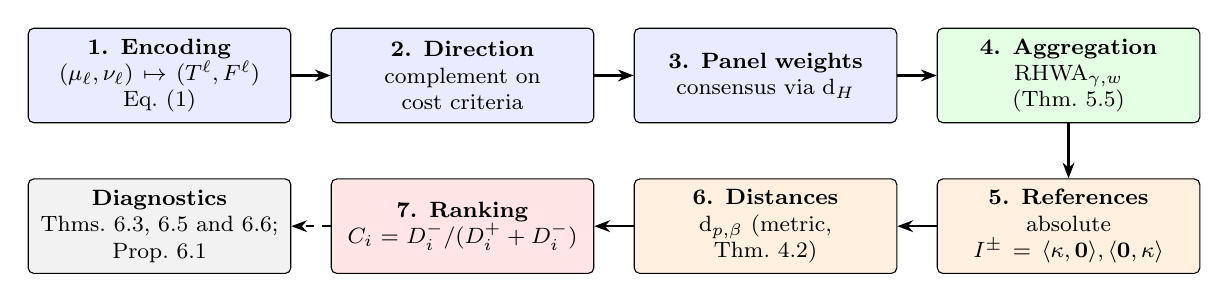
\begin{tikzpicture}[node distance=4mm and 5mm,
  box/.style={draw, rounded corners=2pt, align=center, minimum height=12mm, text width=31mm, font=\footnotesize, fill=#1},
  box/.default=white, arr/.style={-{Stealth[length=2mm]}, thick}]
\node[box=blue!8] (a) {\textbf{1. Encoding}\\ $(\mu_\ell,\nu_\ell)\mapsto(T^\ell,F^\ell)$\\ Eq.~(1)};
\node[box=blue!8, right=of a] (b) {\textbf{2. Direction}\\ complement on\\ cost criteria};
\node[box=blue!8, right=of b] (c) {\textbf{3. Panel weights}\\ consensus via $\dd_H$};
\node[box=green!10, right=of c] (d) {\textbf{4. Aggregation}\\ $\HWA_{\gamma,w}$\\ (Thm.~5.5)};
\node[box=orange!12, below=7mm of d] (e) {\textbf{5. References}\\ absolute $I^\pm=\langle\kappa,\mathbf0\rangle,\langle\mathbf0,\kappa\rangle$};
\node[box=orange!12, left=of e] (f) {\textbf{6. Distances}\\ $\dd_{p,\beta}$ (metric,\\ Thm.~4.2)};
\node[box=red!10, left=of f] (g) {\textbf{7. Ranking}\\ $C_i=D^-_i/(D^+_i+D^-_i)$};
\node[box=gray!10, left=of g] (h) {\textbf{Diagnostics}\\ Thms.~6.3, 6.5 and 6.6;\\ Prop.~6.1};
\draw[arr] (a)--(b); \draw[arr] (b)--(c); \draw[arr] (c)--(d); \draw[arr] (d)--(e); \draw[arr] (e)--(f); \draw[arr] (f)--(g); \draw[arr,dashed] (g)--(h);
\end{tikzpicture}
\end{document}
